\documentclass[12pt, twoside]{article}
\usepackage[francais]{babel}
\usepackage[T1]{fontenc}
\usepackage[latin1]{inputenc}
\usepackage[left=6mm, right=6mm, top=3mm, bottom=3mm]{geometry}
\usepackage{float}
\usepackage{graphicx}
\usepackage{array}
\usepackage{multirow}
\usepackage{amsmath,amssymb,mathrsfs}
\pagestyle{empty}
\begin{document}



\section*{\center{Aide individualis�e: la r�daction}} 



\subsection*{QCM sur la r�daction}
Toutes les r�sultats aux questions suivantes sont justes, mais la
justification et la r�daction ne sont pas toujours correctes et sont parfois
insuffisantes. Le but est de trouver la ou les bonnes justifications
(r�dactions) pour chaque question. Cocher la ou les r�ponses qui sont bien
r�dig�es.

\begin{enumerate}
  \item Quelle est la nature de $\dfrac{7}{8}$?
  
  
  \enskip
  \begin{tabular}{|m{6cm}|c|}
  \hline
 La nature de $\dfrac{7}{8}$ est un rationnel &   \\[4mm]
  
  \hline
   $\dfrac{7}{8} \in \mathbb{Q}$ &  \\[4mm]
 
  \hline
  $\dfrac{7}{8}$ est un rationnel & \\[4mm]

  \hline
  $\dfrac{7}{8}$ est de nature rationnel & \\[4mm]

  \hline
  \end{tabular}

\enskip
\item Calculer le $pgcd$ de $126$ et de $224$.
 \bigskip
 
 
  \begin{tabular}{|c|c|}
  \hline
 $pgcd(126,224)=14$ &   \\[2mm]
  
  \hline
  \begin{tabular}{cc}
   \begin{minipage}{2cm}
  \begin{tabular}{c|c}
  $126$ & \fbox{$2$} \\
  $63$ & $3$ \\
  $21$ & $3$\\
  $7$ & \fbox{$7$} \\
  $1$ &  \\
 
  \end{tabular}
  \end{minipage}
&



\begin{minipage}{2cm} \medskip
\begin{tabular}{c|c}
$224$ & \fbox{$2$} \\
$112$ & $2$\\
$56$ & $2$\\
$28$ & $2$\\
$14$ & $2$\\
$7$ & \fbox{$7$}\\
$1$ & \\

\end{tabular}

\end{minipage}\\
Donc $pgcd(126,224)=2 \times 7=14$
 \end{tabular} &  \\[4mm]
 
  \hline
  $126=2 \times 3^{2} \times$ et $224= 2^{5} \times 7$ donc $pgcd(126,224)=2
  \times 7=14$  & \\[2mm]

  \hline
  La calculatrice donne $14$ & \\[2mm]

  \hline
  \end{tabular}

\bigskip
\item $101$ est-il premier? 
 
 
 \enskip
  \begin{tabular}{|m{14cm}|c|}
  \hline
 $2, \ 3, \ 5$  et $7$ ne divisent pas $101$ donc $101$ est premier. &   
 \\[2mm]
  
  \hline
  $2, \ 3, \ 5$  et $7$ ne divisent pas $101$ et $101:11\approx 9<11$ donc
  $101$ est premier. &
  \\[2mm]
 
  \hline
  $101$ est divisible seulement par $1$ et lui m�me donc $101$ est premier.&
  \\[2mm]

  \hline
  J'ai test� tous les entiers comris entre $2$ et $100$, ils ne divisent pas
  $101$ donc $101$ est premier. &
  \\[2mm]

  \hline
  \end{tabular}
\end{enumerate}


\subsection*{La r�daction en g�om�trie}

On rappelle les th�or�mes de g�om�trie suivants (ceux sont les seuls � utiliser
pour les deux exercices qui suivent):
\bigskip

\textbf{Th�or�me}: Si $[AB]$ est un diam�tre d'un cercle $\mathcal{C}$ et si $M$
est un point de $\mathcal{C}$ (diff�rent de $A$ et $B$) alors $ABM$ est
rectangle en $M$.

\enskip

\textbf{Th�or�me}: Si deux droites du plan sont perpendiculaires � une m�me
troisi�me alors elles sont parall�les entre elles.

\enskip

\textbf{Th�or�me}: La droite qui passe par le milieu d'un c�t� d'un triangle et
qui est parall�le � un autre c�t� passe par le milieu du troisi�me c�t�.

\enskip 

\textbf{Th�or�me}: Les trois hauteurs d'un triangle sont concourantes. 

\begin{center}
	  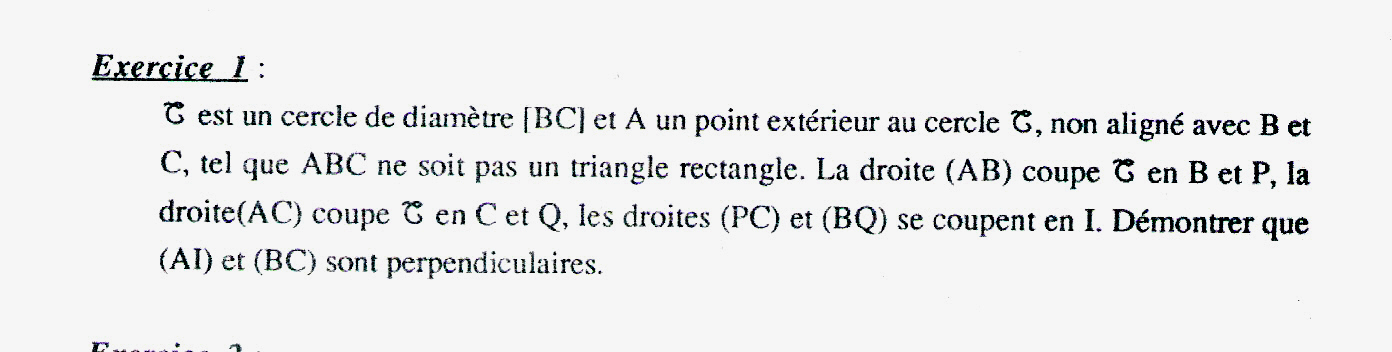
\includegraphics[width=20cm]{images/ex3.jpg} 
\end{center} 
\begin{center}
	  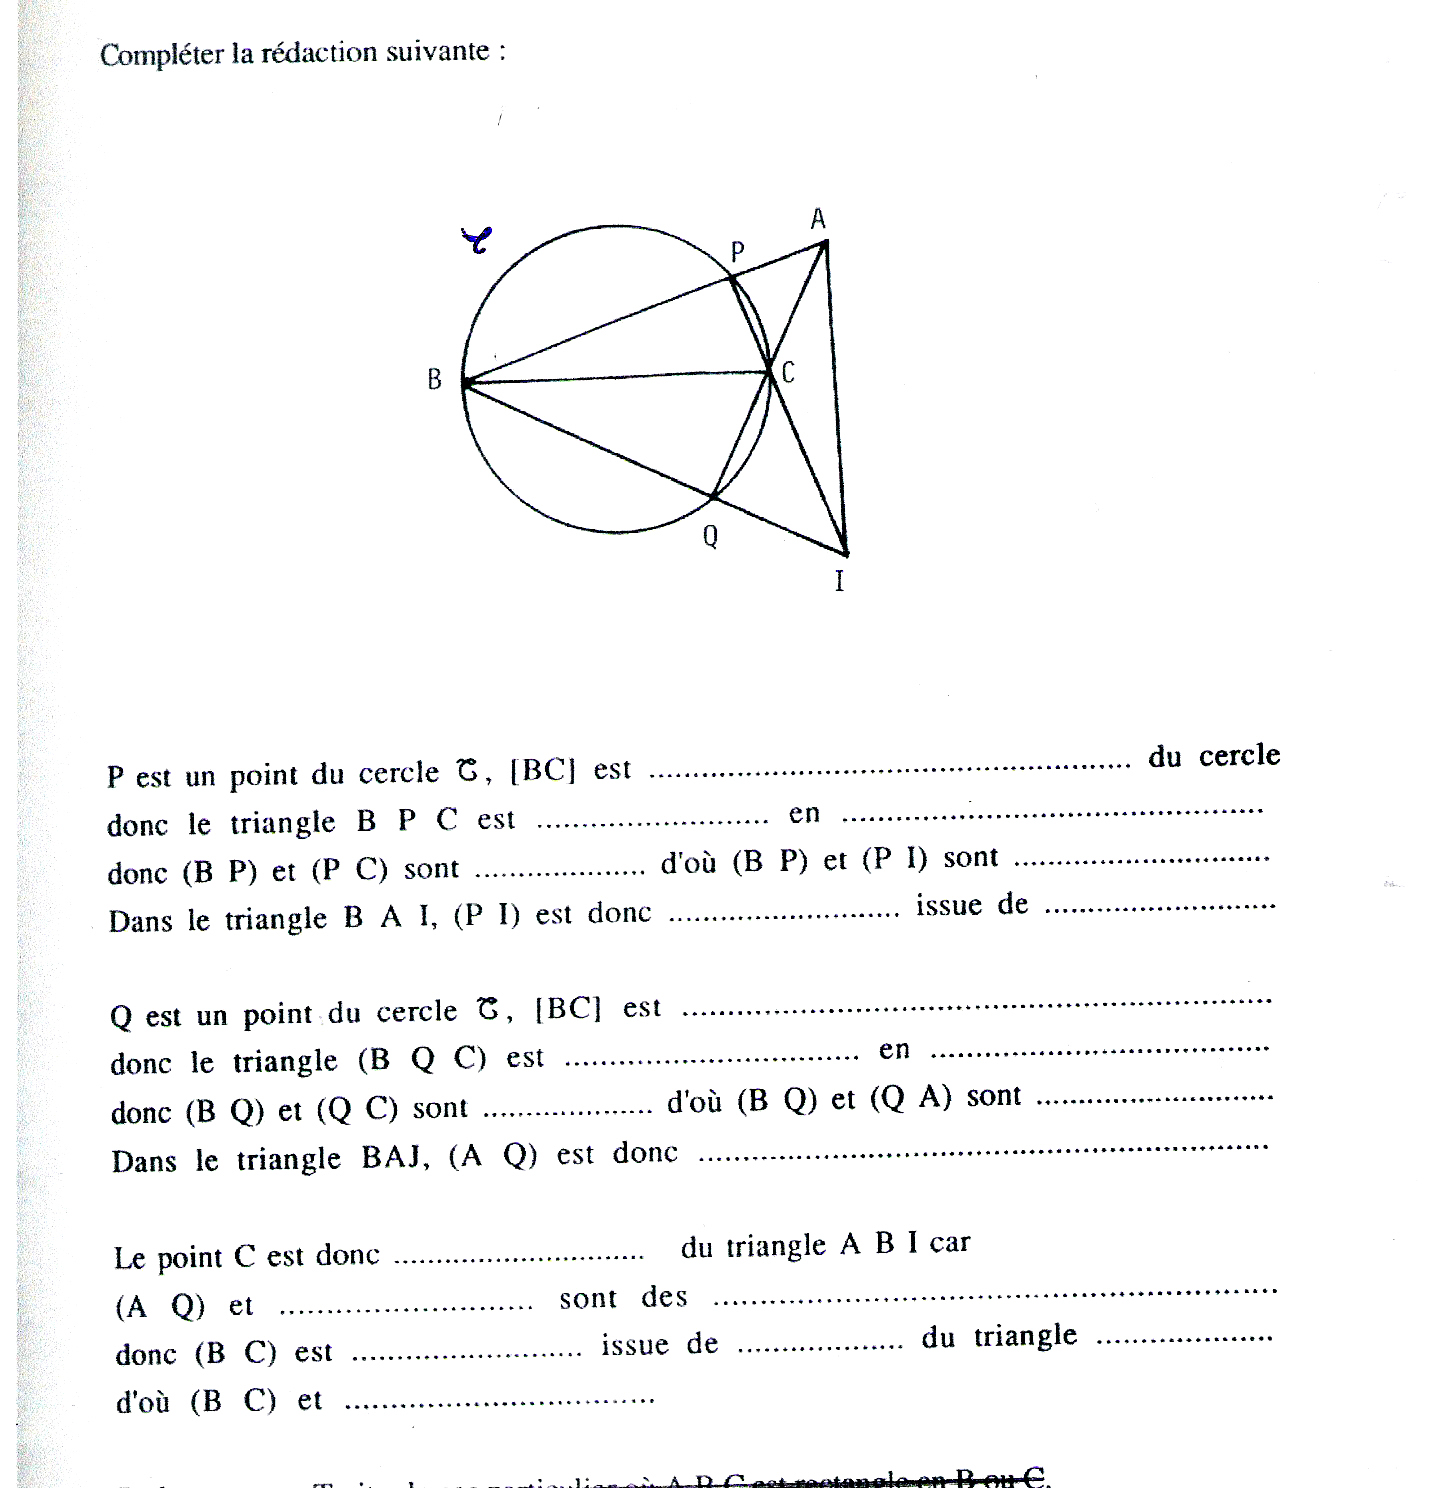
\includegraphics[width=17cm]{images/ex1.jpg} 
\end{center}
\begin{center}
	  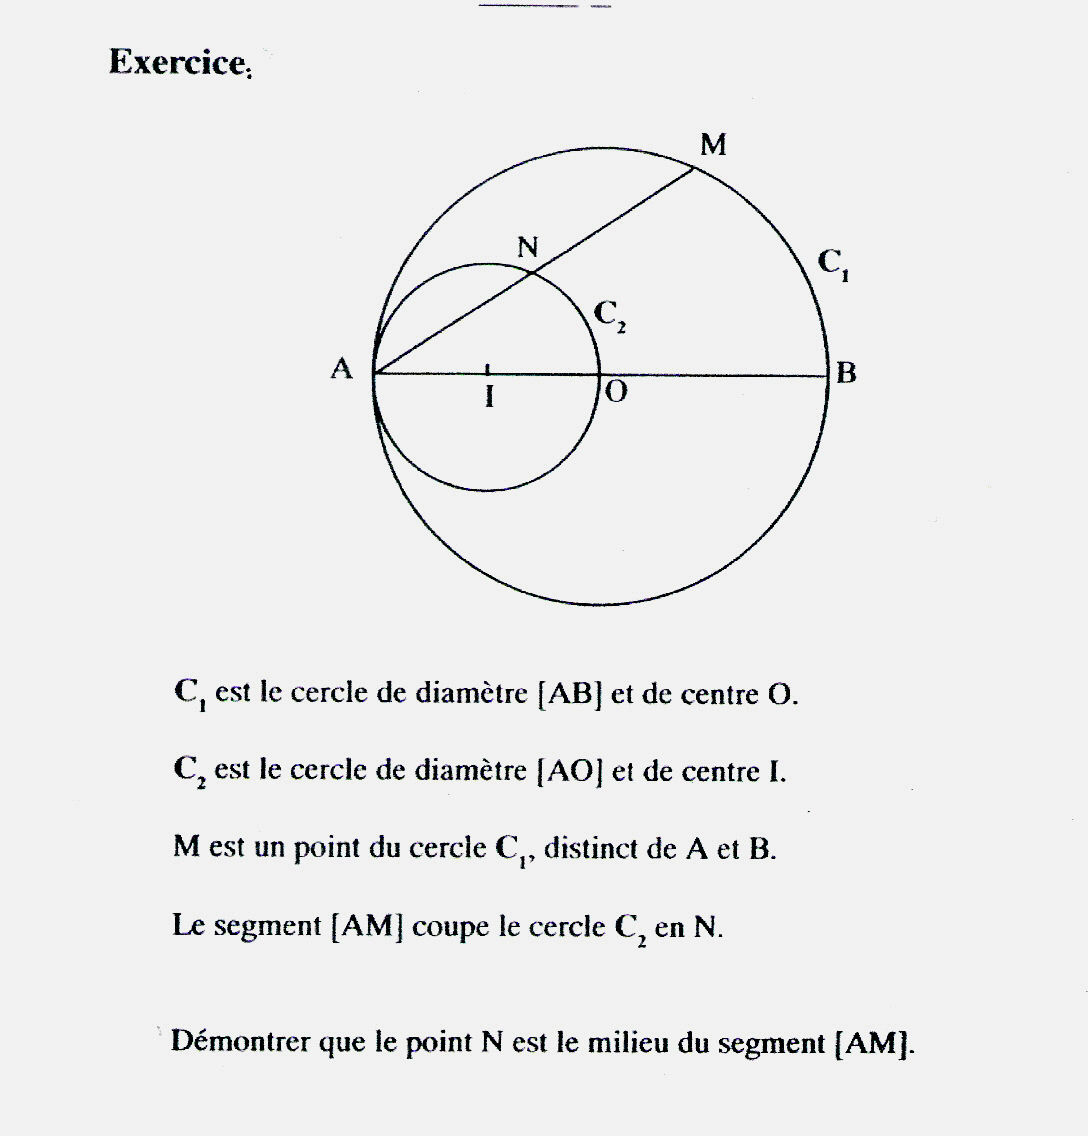
\includegraphics[width=15cm]{images/ex2.jpg} 
\end{center}
\end{document}
